\begin{figure}
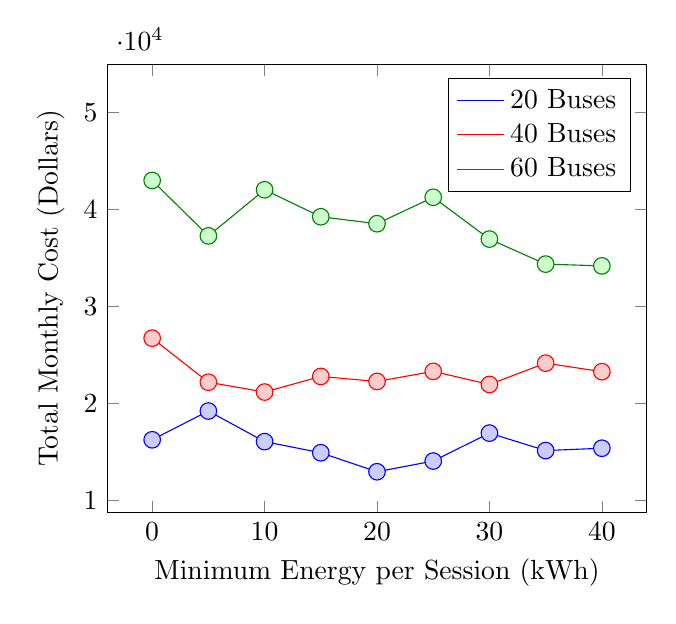
\begin{tikzpicture}
\begin{axis}[xlabel=Minimum Energy per Session (kWh), ylabel=Total Monthly Cost (Dollars), ymax=55000, legend pos=north east]
	\addplot[blue] coordinates {
		(0, 16256.21)   
	  (5, 19221.75)  
		(10,16068.21)  
		(15,14919.20)  
		(20,12958.06)  
		(25,14062.05)  
		(30,16946.17)  
		(35,15143.95)  
		(40,15386.03)};
\addplot[red] coordinates {
		(0, 26738.71)
		(5, 22196.87) 
	  (10,21180.43)
		(15,22789.78)
		(20,22273.05)
		(25,23312.12)
		(30,21963.29)
		(35,24164.56)
		(40,23282.00)};
\addplot[green!50!black] coordinates {
		(0, 43007.78)
		(5, 37289.58)
	  (10,42044.81)
		(15,39261.70)
		(20,38546.15)
		(25,41271.99)
		(30,36959.39)
		(35,34377.97)
		(40,34195.29)}; 
\addplot[blue!20, draw=blue, only marks, mark size=3pt] coordinates {
		(0, 16256.21)   
	  (5, 19221.75)  
		(10,16068.21)  
		(15,14919.20)  
		(20,12958.06)  
		(25,14062.05)  
		(30,16946.17)  
		(35,15143.95)  
		(40,15386.03)};
\addplot[red!20, draw=red, only marks, mark size=3pt] coordinates {
		(0, 26738.71)
		(5, 22196.87) 
	  (10,21180.43)
		(15,22789.78)
		(20,22273.05)
		(25,23312.12)
		(30,21963.29)
		(35,24164.56)
		(40,23282.00)};
\addplot[green!20, draw=green!50!black, only marks, mark size=3pt] coordinates {
		(0, 43007.78)
		(5, 37289.58)
	  (10,42044.81)
		(15,39261.70)
		(20,38546.15)
		(25,41271.99)
		(30,36959.39)
		(35,34377.97)
		(40,34195.29)}; 
\legend{20 Buses, 40 Buses, 60 Buses} 
\end{axis}
\end{tikzpicture}
\caption{Cost comparison of different degragmentation thresholds in a pro-schedule optimization scheme.}
\label{fig:results:costDefragmentationProTime}
\end{figure}
